En este trabajo comenzamos tomando un dataset con el objetivo de elaborar un primer modelo de predicción. Los resultados iniciales no fueron satisfactorios, y empezamos a evaluar distintas alternativas para mejorarlos. En este sentido generamos un nuevo dataset con un número mucho mayor de variantes. Este nuevo dataset no derivó en una mejora sustancial, si comparamos los resultados del dataset Físico-Químico con los obtenidos en el dataset VarQ Curado. Luego exploramos nuevas dimensiones que el dataset original no poseía. Estas nuevas variables genómicas si representaron una mejora sustancial con el dataset Físico-Químico, y estas mejoras se mantuvieron al sumarlas al dataset original. Estas mejoras pueden observarse en las figuras \ref{fig:curvas_auc_humsavar} y \ref{fig:curvas_auc_varq}. En particular las variables que aportaron las mejoras más significativas son las de conservación a nivel filogenético como también las matrices de sustitución de aminoácidos.

\subsection{Trabajo Futuro}

Uno de los principales productos de este trabajo es la generación de un nuevo dataset que contiene numerosas variables estructurales y físico-químicos de la proteína, sumados a variables de tipo genómico. Este dataset también contiene variantes que están ligados a diferentes genes, que a su vez poseen cantidades distintas de SNPs potencialmente dañinos. Una de los trabajos que quedaron pendientes consisten en generar modelos individuales para cada gen, dado que puede existir un sesgo en nuestro modelo en caso de tener un número muy grande de SNPs de un gen determinado.

También creemos que los trabajos futuros que deriven de este deberían hacer énfasis en la generación de modelos que mejoren la selección de hiperparámetros (en particular sugerimos el uso de técnicas de optimización bayesiana), y un tratamiento de nulos en variables categóricas más avanzado en comparación al usado en este trabajo. 


\newpage



\begin{figure}[H]
\centering
\begin{subfigure}[b]{0.6\textwidth}
    \centering
    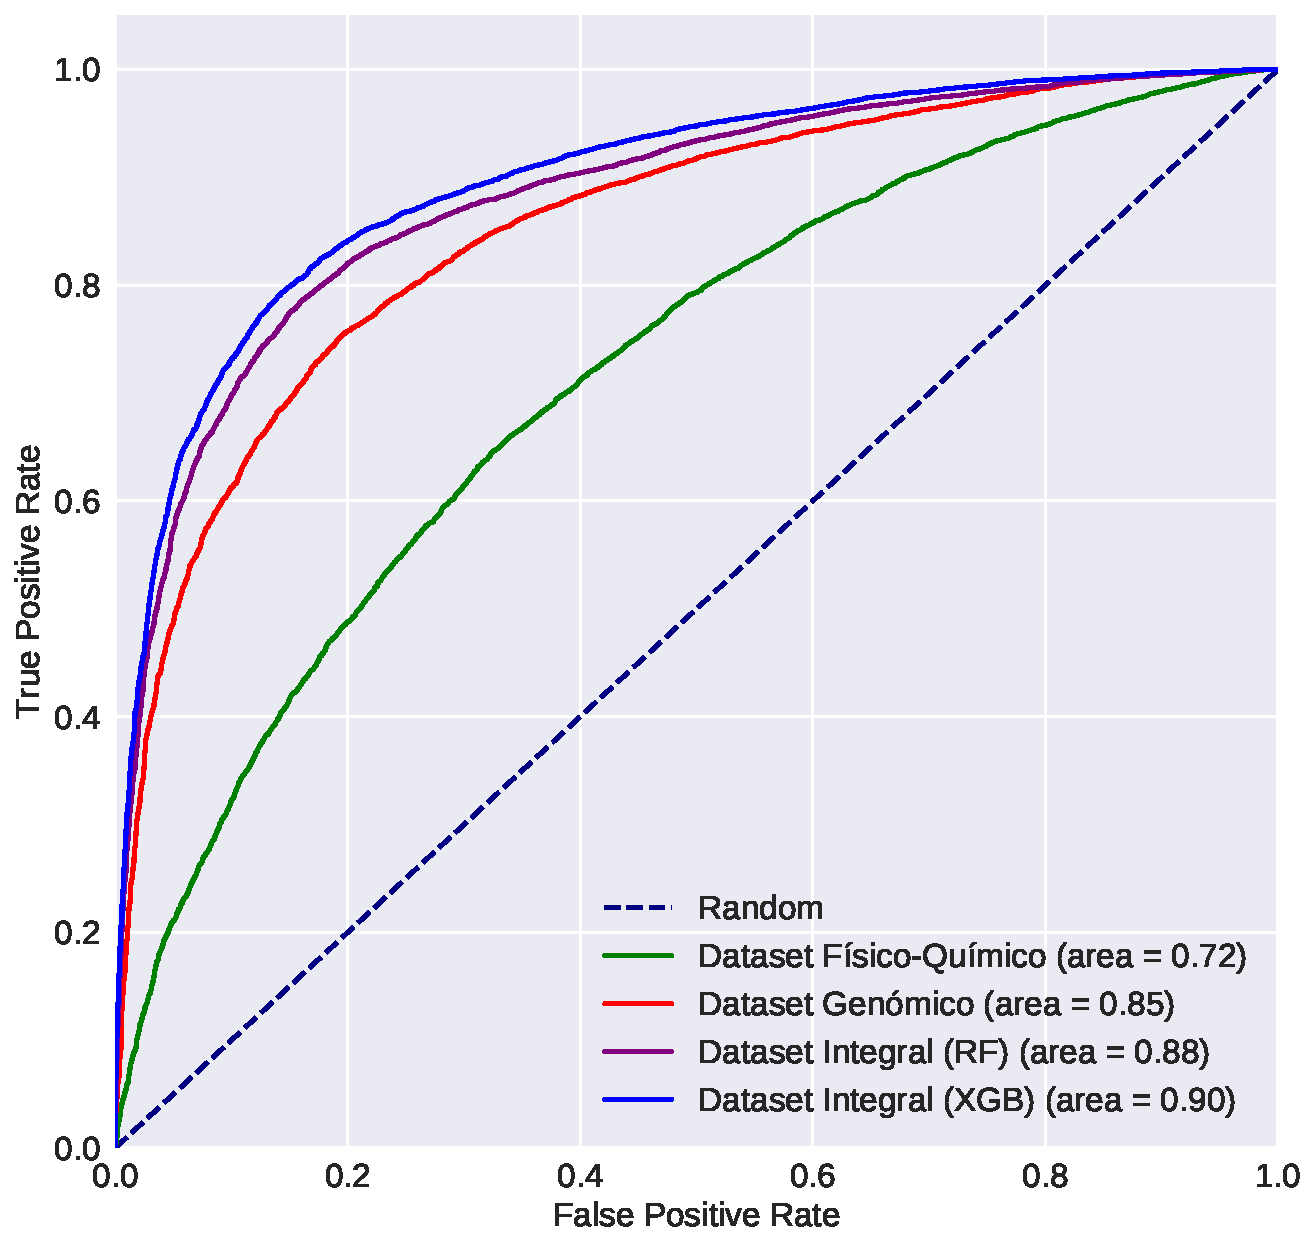
\includegraphics[width=\textwidth]{documents/latex/figures/4/curvas_auc_humsavar.pdf}
    \caption{Comparación de curvas ROC entre los datasets Físico-Químico, Genómico e Integral.}
    \label{fig:curvas_auc_humsavar}
\end{subfigure}

\hfill
\hfill

\begin{subfigure}[b]{0.6\textwidth}
    \centering
    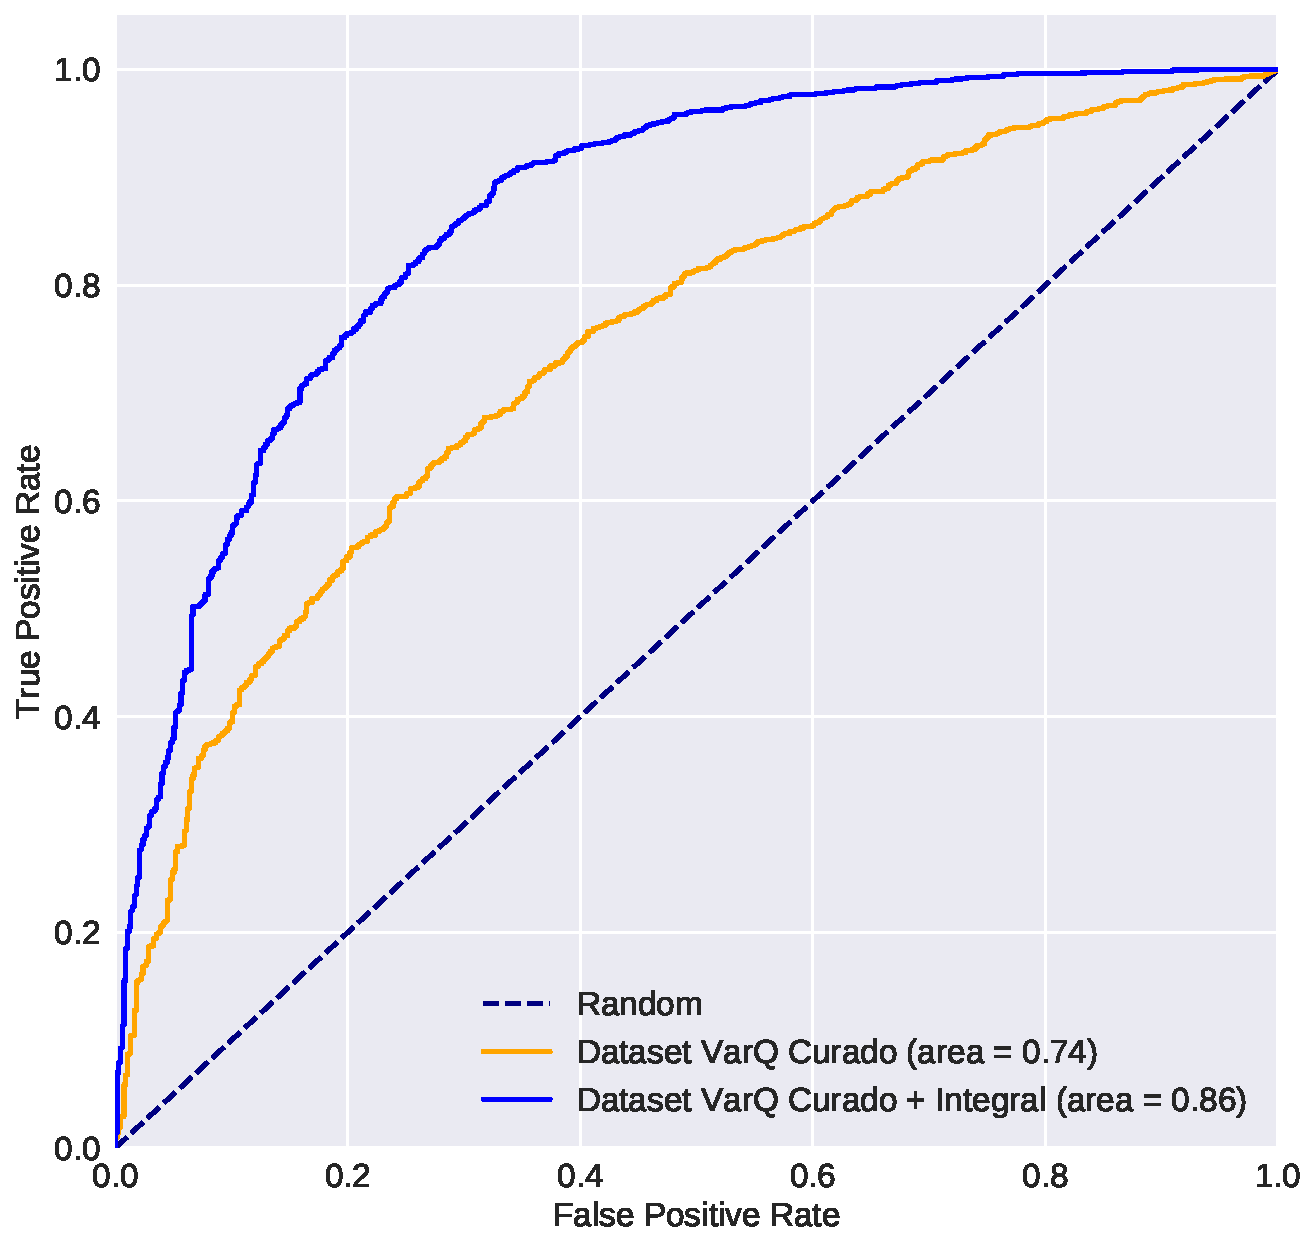
\includegraphics[width=\textwidth]{documents/latex/figures/4/curvas_auc_varq.pdf}
    \caption{Comparación de curvas ROC entre los datasets VarQ Curado y VarQ Curado + Integral.}
    \label{fig:curvas_auc_varq}
\end{subfigure}

\end{figure}


